%
% File acl2018.tex
%
%% Based on the style files for ACL-2017, with some changes, which were, in turn,
%% Based on the style files for ACL-2015, with some improvements
%%  taken from the NAACL-2016 style
%% Based on the style files for ACL-2014, which were, in turn,
%% based on ACL-2013, ACL-2012, ACL-2011, ACL-2010, ACL-IJCNLP-2009,
%% EACL-2009, IJCNLP-2008...
%% Based on the style files for EACL 2006 by 
%%e.agirre@ehu.es or Sergi.Balari@uab.es
%% and that of ACL 08 by Joakim Nivre and Noah Smith

\documentclass[11pt,a4paper]{article}
\usepackage[hyperref]{acl2018}
\usepackage{times}
\usepackage{latexsym}
\usepackage{graphicx}
\usepackage{url}

\aclfinalcopy % Uncomment this line for the final submission
%\def\aclpaperid{***} %  Enter the acl Paper ID here

%\setlength\titlebox{5cm}
% You can expand the titlebox if you need extra space
% to show all the authors. Please do not make the titlebox
% smaller than 5cm (the original size); we will check this
% in the camera-ready version and ask you to change it back.

\newcommand\BibTeX{B{\sc ib}\TeX}

\title{Detecting Sarcasm Using Attention-Based Convolutional Neural Networks}

\author{Saul Grimaldo \\
  DATASCI W266\\
  UC Berkeley \\
  School of Information \\
  {\tt saul\char`_grimaldo@berkeley.edu} \\\And
  Ramsey Maga{\~n}a \\
  DATASCI W266\\
  UC Berkeley \\
  School of Information \\
  {\tt ramagana@berkeley.edu} \\}

\date{}

\begin{document}
\maketitle
\begin{abstract}
Due to the increasing importance of NLP, it's important now more than ever to detect linguistic phenomena that can often be subtle but which ignoring may result in costly mistakes in critical business usages. This paper attempts to provide a practical way of detecting sarcasm, a subtle linguistic phenomenon that often completely changes the meaning of the language used. 

We provide some background on models that are typically used for sarcasm detection which heavily rely on information that may be difficult to obtain for the typical business as well as some neural network based models that attempt to use only messages posted within the same general context. In our case, we focus on messages in a Twitter message thread. This algorithm will also generate word embeddings that with additional work may improve the ability to detect sarcasm without requiring the use of new models.
\end{abstract}

\section{Introduction}
Sarcasm is challenging to detect. Even the typical person may have difficulties distinguishing a non-sarcastic comment from a sarcastic one. Often times, a person requires context on the conversation to be able to confidently determine whether a statement is sarcastic. This makes sarcasm even more difficult for a machine learning algorithm to detect. However, sarcasm detection is critical in some applications. 

The field of sentiment analysis can often be critical for business attempting to grow using customer testimony to present prospective customers with happy users experience with their products. A sarcastic message may, however, slip through the cracks, providing a scathing review hidden by heavy sarcasm that uses highly positive language. Sarcasm is also important in detecting toxic messages. Often times toxic messages are delivered using sarcastic comments. In both cases, it's possible to use the immediate context without having to rely on user-level data.

Current techniques rely heavily on user history. That is, we must understand the user who's posting a message to understand if they are
being sarcastic. Some algorithms even require knowledge of the target audience as well. Properly capturing this information however, may be unwieldy and perhaps even unethical. 

We present a methodology that uses convolutional neural networks that rely only on the context in which the message was posted. We define context in two ways. First is what, if anything, a given tweet is responding to. To do this, we collected the immediately prior tweet to which the twitter message of interest is responding to if they were responding to anything. The second definition of context is the given topic that the tweet is covering. In twitter, we can gather this sort of contextual information through the use of hashtags.

We rely on data scraped through Twitter to build our models, using the \#sarcasm and \#sarcastic hashtags to label our training examples. We sample a set of popular hashtags as well to gather negative examples. This provides a fundamental issue. It's common for people to be sarcastic without using a hashtag announcing the fact. It's also possible that someone uses the sarcasm or sarcastic hashtags even when they are not being sarcastic. As such, our algorithm will  be built on an imperfect foundation. To more properly build this model out would require a team of annotators to determine whether a given tweet is sarcastic. However, even this method proved to be challenging for Davidov et al as their team of expert annotators were not completely certain whether a message should be labeled as sarcastic [1].

\section{Background}

Historical experiments in this space have sourced data from social media channels like twitter, utilizing hashtags for labeling sarcasm (e.g. \#sarcasm, \#sarcastic, \#not) as seen in the paper by Bamman and Smith. In the Bamman paper, logistic regression is used for classification by training the model with a combination of tweet, author and environmental features[2].  In a paper by Amir et al[3] they use user embeddings to help provide contextual features for their model.  Moreover, there have been more advanced approaches to detecting sarcasm by way of using CNNs + LSTM + DNN as seen in Ghosh and Veale[4].  Additionally some semi-supervised approaches are also used as done by Davidov et al[1]. We compare the performances of these models against ours in the results section.

\section{Methods}
Our objective is to predict whether a message is sarcastic or not. To measure the effectiveness of our methodology, we will be using the  F1-score , in a similar way as the authors discussed in the background section. 

Two key techniques are used to detect whether a given tweet is sarcastic or not: the baseline model, which is a Naive Bayes model using a bag of words, and the Bi Convolutional Neural Network model,  which uses the message of interest, and the message which is being responded to as the main set of features.

For the purpose of these experiments, a 60-30-10 training-validation-test split is performed on our data. 

\subsection{Data}
Similar to both the Ghosh \& Veale and the Bannam \& Smith papers, we utilize functionality provided by twitter to access twitter streams. Using the twitter streaming api for python, tweepy, we collect our positive and negative class examples, sarcastic and non-sarcastic respectively.  

To collect positive examples of sarcasm we used self-declared labels of sarcasm with the following the \#sarcasm and \#sarcastic hashtags.  To collect negative examples of sarcasm we aimed to create sample that is representative of the Twitterspere population. Our negative hashtags were chosen by identifying the most active hashtags for the following categories:  gaming, sports, fun, science, non-profit, news, technology, music, politics, and lifestyle.  Across the 10 categories, we have included in 194 unique hashtags in the filter the stream to collect the negative class.  

The tweet objects are received in JSON-like objects.  Features of the tweets that were of interest include user identification information, full text of the tweet including the hashtag labels, information connecting the tweet to any tweet (or status) and user that it is in reply to.  Lastly, additional attribute information to filter data set, such as language and geographical information. 

As sarcasm is a tricky classification and has inherent grounding issues, we sought to incorporate the previous tweet in the thread that our current data point is in response to.   Although, the objects obtained from twitter stream does have the user and status of the post it is in response to, it does not contain the previous status content itself.  Despite limitations of the api, we are able to use user\_id and status\_id to reconstruct url and scrape and parse the previous tweets. 

\subsection{Data Exploration}
To enforce class balance, we ensured that there were equal number of sarcastic and non-sarcastic tweets in our training set. A total of about 12,000 tweets were used in our modeling processes.

Examples of sarcastic comments include:
 "Good job @GOP, good job..." in response to a tweet mentioning that a Holocaust denier was nominated by the GOP.   
 
 "Nothing like this beautiful first day of spring!!! \#sarcasm \#itssnnowing \#sadsies". 
 
 In one case, the message is congratulating the GOP for something many may consider a heinous act, and the second is immediately negating her happiness with the weather with a "sadsies" hashtag. In the first case, a message that elicited a highly negative response is being met with a positive message and the second tweet immediately negates the general sentiment of the message within the hashtags. We are hoping that the methodology being used will be able to detect these dramatic changes in sentiment and use them as a way to predict whether or not something may be sarcastic in nature.

Below is a histogram of token count per tweet.

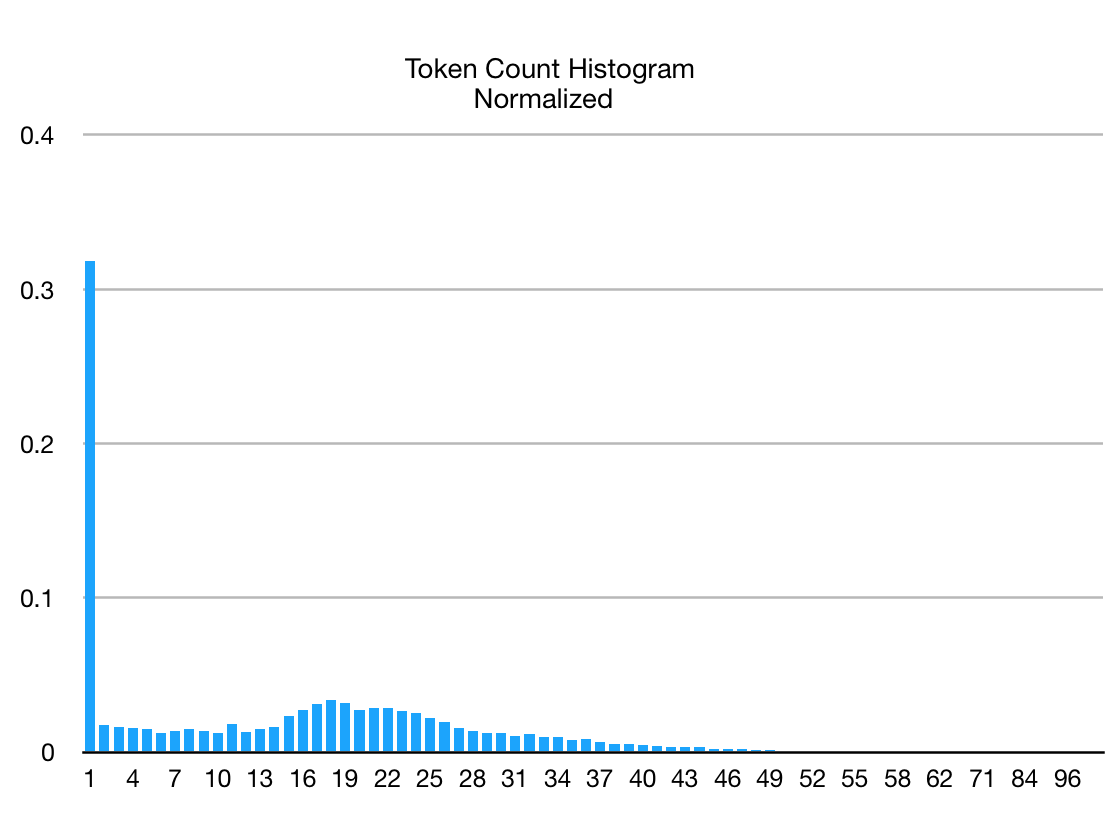
\includegraphics[width=75mm,scale=0.5]{tokenhistogram.png}

We can see above that, generally speaking we can contain the full content of a tweet distilled into a set of 40 tokens (97\% of tweets contained less than 40 tokens), but to be conservative we assumed a tweet length of 40 tokens. For the CNN model, this allowed us to pad our tweets with a "PADDING" token to ensure consistent tweet length. Tweets longer than 40 tokens were truncated.

\subsection{Defining our Vocabulary}

To define our vocabulary we took two main approaches. The key difference in the approach was the treatment of hashtags. In one version, hashtags were tokenized as separate tokens. This allows us to capture additional context that may not be available in using only the prior tweet. To confirm that this methodology helped improve accuracy of our model, we also mapped all hashtags to a single token, which we named "HASHTAG". 

Under both methodologies, we tokenized all URLs as "LINK" tokens, retweet tags (including username attached to that retweet as "retweet", all remaining usernames as "USERNAMES", and finally each digit in a number as DG. 

We tuned the vocabulary length using the CNN model to decide on optimal vocabulary size. To that end, we relied on a vocabulary of only 2,500 words. This is likely driven by the relatively small size of the dataset we built. With a larger dataset, we'll likely be able to improve the accuracy of our models with a larger vocabulary as we will be less likely to run into overfitting issues.

\subsection{Baseline}
A baseline model was built using a word count based multinomial Naive Bayes bag of words model with Laplace smoothing. The bag of words used was defined using the methodology described above. 

\subsection{Bi Convolutional Neural Network Model}

A model was implemented that uses an architecture proposed by Yin et. al [5]. The model is as follows. Two separate CNN processes are run where one processes the context sentence and the other processes the tweet of interest. An embedding layer generates an embedding vector for each token in our vocabulary. This embedding layer is shared between the two CNN processes. We opted against pre-trained word vectors as we wanted to capture the dynamic nature of twitter tweets as well as generate word vectors for hashtags and emojis. 

Each set of word vectors is then concatenated together and is then passed through the convolutional layer. By padding our tweets, we effectively have what is a variation of the wide variation. This variation generates an embedding for the "PADDING" token instead of a 0 embedding. The convolution layer also allows for the sharing of the convolution weights across the two processes. A tanh activation function of the form tanh(W*c + b)  where c is the concatenated word vectors, W is the convolution weights, and b the bias is used. Similar to Yin et. al, we use an average pooling layer that results in a tweet embedding vector of the same size as the word embedding vectors. The two resulting tweet vectors are concatenated together, and a logistic regression output layer is applied to the concatenated word vectors.

A diagram describing this procedure is below.

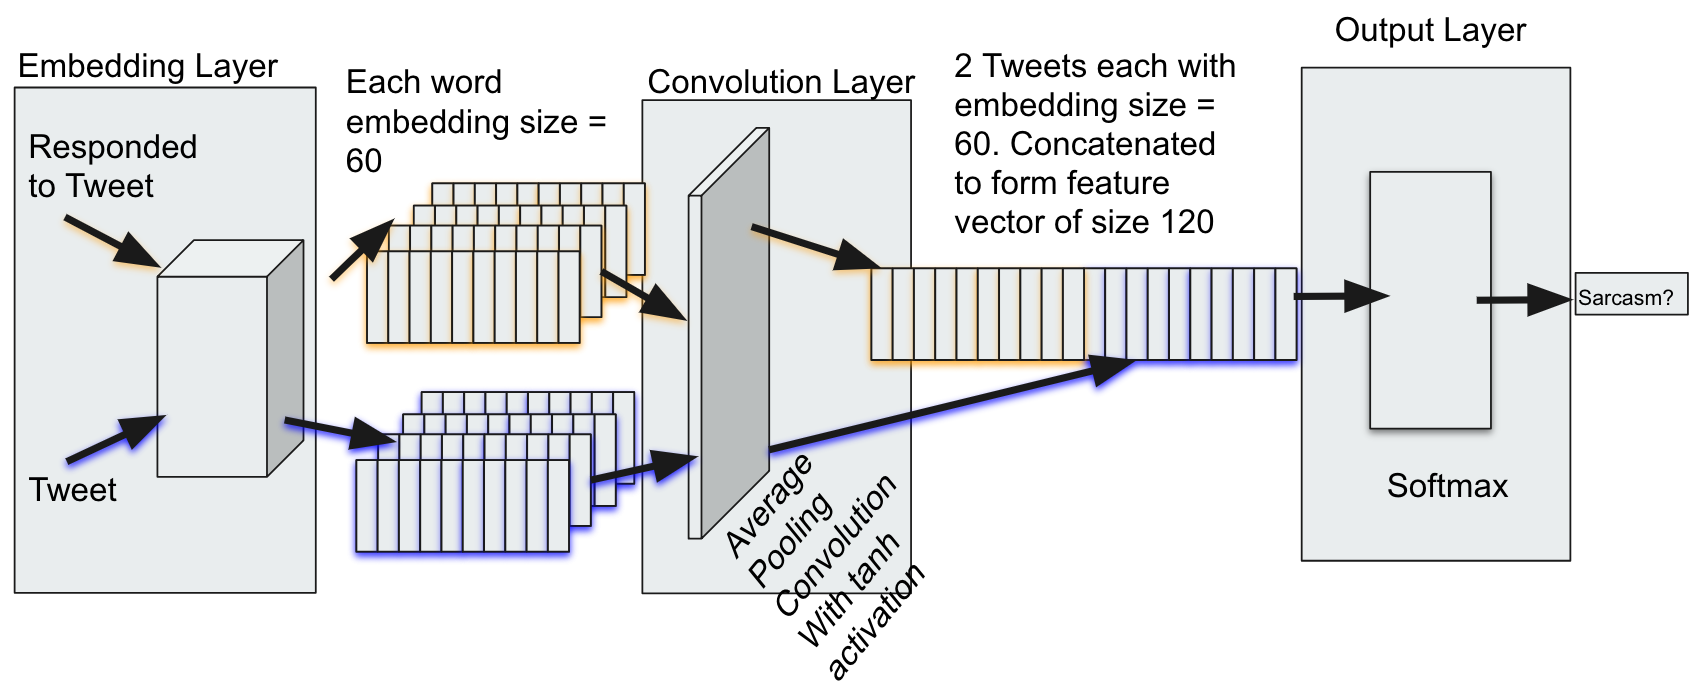
\includegraphics[width=75mm,scale=0.5]{bcnn.png}


\section{Results and Error Analysis}

A comparison of the different models we built as well as the best models proposed by the authors discussed in the background research section can be seen below.

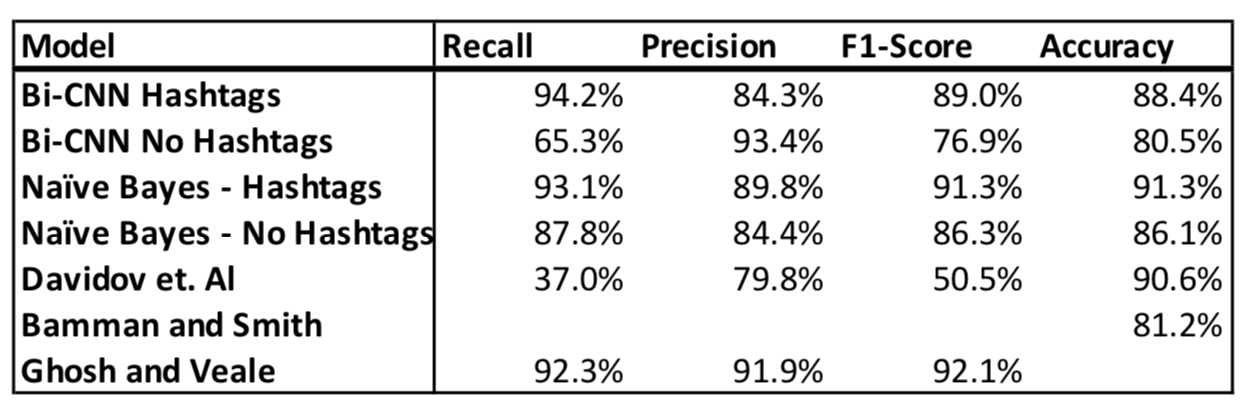
\includegraphics[width=75mm,scale=0.5]{results.png}

Our Naive Bayes algorithm outperformed our Bi CNN model as well as most of the works presented by the authors described.

To check for common errors, we looked at the top 5 tweets that our model got most wrong. The method for this was simple. For the CNN model we looked at the difference in the logits and ranked each tweet this way, while for the Naive Bayes model we used the differences int he log probabilities. 

Common errors existed within all 4 of the models we built. One common tweet that was incorrectly tagged as sarcastic is "what is with that? theyre only going to blame the guns now? no people? at all? oh yeah they will blame trump. there is no agenda though..."

This tweet manifests a fundamental problem with our tagging of sarcastic tweets. The message does seem to be sarcastic, especially the last two sentences in the tweet. This is an example of a tweet that our model tagged correctly, was incorrectly classified as an error due to issues with our methodology for finding sarcastic tweets. 

Our models which mapped all hashtags to a single "HASHTAG" token resulted in being overconfident in tweets where a large number of tweets were present in the tweet, an issue we attempted to remedy by mapping each hashtag to its own token, but due to the smaller vocabulary we relied on due to the limitations resulting from the size of our data, our model continued being overconfident with tweets made up of mostly hashtags. Still, this increased our accuracy and f1-score considerably at the cost of precision.

It's unsurprising that our Naive Bayes models outperformed our BiCNN models. Our data set was relatively small, and we relied on relatively small word embedding sizes. Furthermore, the Naive Bayes algorithm is able to simply identify the hashtags that were used to generate the negative samples. Still the model continued to perform extremely well on the test set even without keeping the hashtags as their own separate token. However, we believe that this is likely driven by the fact that our models might simply be picking up words idiosyncratic to these hashtags.


\section{Conclusion}



\textbf{References}

[1] http://www.aclweb.org/anthology/W10-2914

[2] https://homes.cs.washington.edu/~nasmith/papers/bamman+smith.icwsm15.pdf

[3] https://arxiv.org/pdf/1607.00976v2.pdf

[4] http://www.aclweb.org/anthology/W16-0425

[5] https://arxiv.org/pdf/1512.05193v3.pdf


\end{document}
